\documentclass{article}
\usepackage{amsmath}
\usepackage{amssymb}
\usepackage{esint}
\usepackage{float}
\usepackage{listings}
\usepackage{graphicx}
\usepackage[font=footnotesize]{caption}
\usepackage[a4paper,top=1cm, bottom=1cm, outer=2.5cm, inner=2.5cm, heightrounded, marginparwidth=5cm, marginparsep=0.5cm]{geometry}

\setlength\parindent{0pt}
\lstset{basicstyle=\footnotesize, frame=single}
\renewcommand{\lstlistingname}{Code}


\begin{document}
\textbf{\Large Home Assignments}
\vspace{0.15cm}

\textbf{\large Digital Signal Processing}

\section*{Introduction}
\paragraph{1. Use Euler's formula to prove that:}

\begin{equation}
	\sin(x) \cos(x) = \frac{1}{2} \sin(2x)
\end{equation}

\paragraph{Given that:}
\begin{align}
	e^{ix} &= \cos(x) + i \sin(x) \label{eq:1}\\
	e^{-ix} &= \cos(-x) + i \sin(-x) = \cos(x) - i \sin(x) \label{eq:2}
\end{align}

\paragraph{Follows:}
\begin{align*}
	\cos(x) &= \frac{e^{ix} + e^{-ix}}{2} & & \text{From adding \ref{eq:1} and \ref{eq:2}}\\
	 \sin(x) &= \frac{e^{ix} - e^{-ix}}{2i} & & \text{From substracting \ref{eq:1} and \ref{eq:2}} 
\end{align*}

\begin{align*}
	\sin(x) \cos(x) &= \frac{e^{ix} + e^{-ix}}{2} \cdot \frac{e^{ix} - e^{-ix}}{2i} & & \text{Substituting \ref{eq:3} and \ref{eq:4}}\\
	&= \frac{e^{i2x} - e^{i0} + e^{i0} - e^{-i2x}}{4i} & & \text{Multiplying fractions}\\
	&= \frac{1}{2} \frac{e^{i2x} - e^{-i2x}}{2i} & & \text{Combining exponentials}\\
	&= \frac{1}{2} \sin(2x) & & \text{Substituting \ref{eq:4}}
\end{align*}


\paragraph{2. Show that:}
\begin{equation}
	\int_0^{T_0} \cos(k \omega_0 t) \cos(n \omega_0 t) dt =
	\begin{cases}
		0,& k \neq n\\
		\frac{T_0}{2},& k = n \neq 0\\
		T_0,& k = n = 0
	\end{cases}
\end{equation}

\paragraph{Given that:}

\begin{equation}
	\cos(x) \cos(y) = \frac{1}{2} \left[ \cos(x-y) + cos(x+y) \right]
\end{equation}

\begin{equation}
	\int_0^{T_0} \cos(k \omega_0 t) dt =
	\begin{cases}
		T_0,& k=0\\
		0,& k \neq 0
	\end{cases}
\end{equation}

\paragraph{Follows:}

\[
	\int_0^{T_0} \cos(k \omega_0 t) \cos(n \omega_0 t) dt 
	= \frac{1}{2} \int_0^{T_0} \left[ \cos\left((k-n)\omega_0 t\right) + \cos\left((k+n)\omega_0 t\right)\right] dt
\]


Case $k \neq n$:

\[
	\frac{1}{2} \int_0^{T_0} \left[ \cos\left(a \omega_0 t\right) + \cos\left(b \omega_0 t\right)\right] dt
	= \frac{1}{2} (0 + 0)
	= 0
\]

Case $k = n \neq 0$:

\[
	\frac{1}{2} \int_0^{T_0} \left[ \cos\left(0\right) + \cos\left(2k\omega_0 t\right)\right] dt
	= \frac{1}{2} T_0 + 0
	= \frac{T_0}{2}
\]

Case $k = n = 0$:

\[
	\frac{1}{2} \int_0^{T_0} \left[ \cos\left(0\right) + \cos\left(0\right)\right] dt
	= \frac{2}{2} T_0
	= T_0
\]


\vspace{0.15cm}
\section*{Fourier Series}
\textbf{3. Show that $B_k = \frac{2}{T_0} \oint f(t) \sin(k \omega_0 t) dt$ is consistent with the Fourier series.}
\\

\textbf{Given that:}

\begin{align}
	\int_{-T_0/2}^{T_0/2} \sin(n \omega_0 t) \sin(k \omega_0 t) dt &=
	\begin{cases}
		0,& k \neq n\\
		\frac{T_0}{2},& k = n \neq 0\\
		T_0,& k = n = 0
	\end{cases}
	\\
	\int_{-T_0/2}^{T_0/2} \cos(n \omega_0 t) \sin(k \omega_0 t) dt &= 0 
\end{align}

\begin{equation}
	\oint \equiv \int_{-T_0/2}^{T_0/2}
\end{equation}

\textbf{Follows:}

\begin{align*}
	B_k &= \frac{2}{T_0} \oint \sum_{n=0}^\infty \left(A_n \cos(n \omega_0 t) + B_n \sin(n \omega_0 t) \right) \sin(k \omega_0 t) dt \\
	&= \frac{2}{T_0} \sum_{n=0}^\infty \left\{A_n \oint \cos(n \omega_0 t) \sin(k \omega_0 t) dt + B_n \oint \sin(n \omega_0 t) \sin(k \omega_0 t) dt \right\} \\
\end{align*}

Case $k = 0$:

\[
	B_0 = \frac{2}{T_0} \sum_{n=0}^\infty \{A_n \underbrace{\oint \cos(n \omega_0 t) \sin(k \omega_0 t) dt}_{=0} + B_n \underbrace{\oint \sin(n \omega_0 t) \sin(k \omega_0 t) dt}_{=0} \} = 0\\
\]

Case $k > 0$:

\[
	B_k = \frac{2}{T_0} \sum_{n=0}^\infty \{A_n \underbrace{\oint \cos(n \omega_0 t) \sin(k \omega_0 t) dt}_{=0} + B_n \underbrace{\oint \sin(n \omega_0 t) \sin(k \omega_0 t) dt}_{=\frac{T_0}{2}} \} = B_k
\]

\textbf{4. Show that $f(t) = \sum_{k=0}^\infty a_k \cos(k \omega_0 t - \phi_k)$ is equivalent to the Fourier series.}
\\

\textbf{Given that:}

\begin{align}
	a &= \sqrt{A^2 + B^2} \\
	\phi &= 
	\begin{cases}
		\arctan(B/A), & A > 0\\
		\pi/2, & A=0, B>0\\
		-\pi/2, & A=0, B<0\\
		\arctan(B/A)+\pi, & A<0, B \geq 0\\
		\arctan(B/A)-\pi, & A<0, B < 0
	\end{cases}
	\\
	\cos(x-y) &= \cos(x)\cos(y) + \sin(x)\sin(y)\\
	\arctan(0) &= 0
\end{align}

\textbf{Follows:}
\\

Case $A>0,\ B=0$:

\begin{align*}
	f(t) &= \sum_{k=0}^\infty a_k \cos(k \omega_0 t - \phi_k) \\
	&= \sum_{k=0}^\infty A_k \cos\left(k \omega_0 t - \arctan{\frac{B}{A}}\right) \\
	&= \sum_{k=0}^\infty A_k \cos(k \omega_0 t) 
\end{align*}

Case $A=0,\ B>0$:

\begin{align*}
	f(t) &= \sum_{k=0}^\infty a_k \cos(k \omega_0 t - \phi_k) \\
	&= \sum_{k=0}^\infty B_k \cos\left(k \omega_0 t - \frac{\pi}{2}\right) \\
	&= \sum_{k=0}^\infty B_k \left[\cos(k \omega_0 t) \cos\left(\frac{\pi}{2}\right) + \sin(k \omega_0 t) \sin\left(\frac{\pi}{2}\right) \right]\\
	&= \sum_{k=0}^\infty B_k \sin(k \omega_0 t) 
\end{align*}
\\

\textbf{5. Consider the triangular function:}

\[
	f(t) = 
	\begin{cases}
		1+\frac{2t}{T},& \text{for} - \frac{T}{2}<t<0\\
		1-\frac{2t}{T},& \text{for} 0\leq t \leq \frac{T}{2}
	\end{cases}
\]

\textbf{a) Derive an algebraic expression for the coefficients $A_k$ and $B_k$ of the Fourier series.}


\begin{align*}
	B_0 &= 0\\
    A_0 &= \frac{1}{T} \int 1 - \frac{2t}{T} dt
    = \frac{1}{T} \left[ t - \frac{t^2}{T} \right]\\
    &= \frac{1}{T} \left[ \frac{T}{2} - \frac{T^2}{4T} \right]
    = \frac{1}{2} - \frac{1}{4} = \frac{1}{4}\\
	a &\equiv k\omega & & \text{Shortening notation}\\
	B_k &= 0\\
	A_k &= \frac{5}{T} \int_0^{T/2} \left( 1-\frac{2t}{T} \right) \cos(at) dt & & \text{Using symmetry and odd property}\\
	&= \frac{4}{T} \int_0^{T/2} \cos(at)-\frac{2t}{T} \cos(at) dt & & \text{Multiplying cosine}\\
	&= \frac{4}{T} \left[ \left[ a^{-1} \sin(at) \right]_0^{T/2} - \int_0^{T/2} \frac{2t}{T} \cos(at) dt \right] & & \text{Computing first integral}\\
	&= \frac{4}{T} \left[ \left[ a^{-1} \sin(at) - \frac{2t}{aT} \sin(at) \right]_0^{T/2} + \int_0^{T/2} \frac{2}{aT} \sin(at) dt \right] & & \text{Applying product rule}\\
	&= \frac{4}{T} \left[ a^{-1} \sin(at) - \frac{2t}{aT} \sin(at) - \frac{2}{a^2T} \cos(at)  \right]_0^{T/2} \\
	&= a^{-1} \sin(aT/2) - 0
		- a^{-1} \sin(aT/2) + 0
		- \frac{2}{a^2T} \cos(aT/2) + \frac{2}{a^2T} & & \text{Inserting boundaries}\\
	&= \frac{4}{k^2\omega^2T^2} [1 - \cos(k\pi) ] & & \text{Replacing} a\\
	&= \frac{1}{k^2\pi^2} [1 - \cos(k\pi) ]
\end{align*}

\newpage

\textbf{b) Plot $A_k$ over $k$ for $0 \leq k < 10$}
\\

\lstinputlisting[language=Python, firstline=0, lastline=13]{code/ex_5.py}

\begin{figure}[H]
	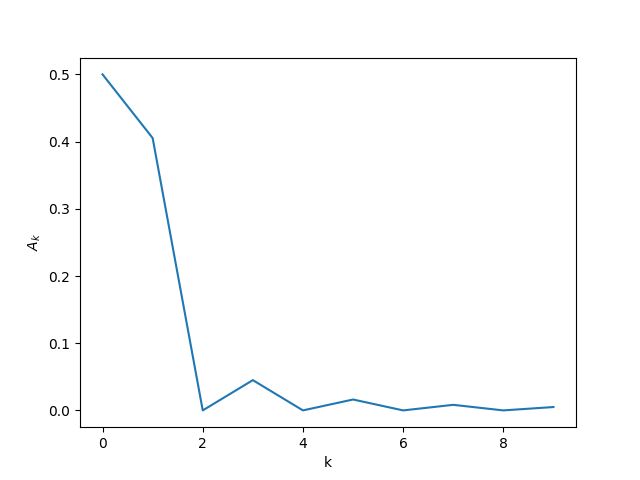
\includegraphics[width=8cm]{img/ex_5_b.png}
	\centering
\end{figure}

\textbf{c) Plot the Fourier series from [-T0;T0] for kmax = 1 and kmax = 9.}
\\

\lstinputlisting[language=Python, firstline=15]{code/ex_5.py}

\begin{figure}[H]
	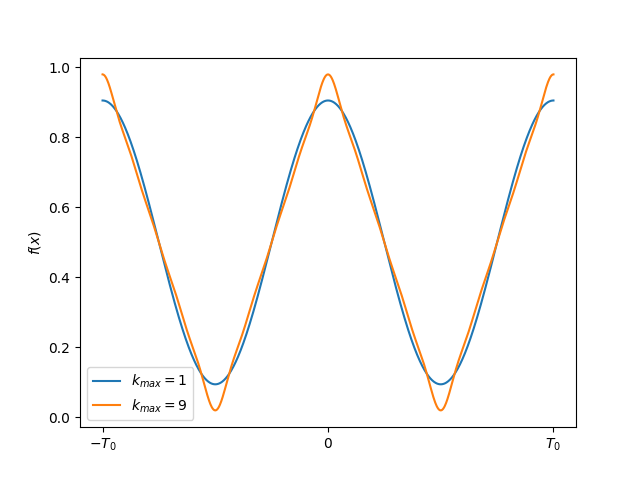
\includegraphics[width=8cm]{img/ex_5_c.png}
	\centering
\end{figure}

\textbf{6. Consider the Fourier series of the rectangular function (see course notes).}

\textbf{a)}

\lstinputlisting[language=Python, firstline=0, lastline=28]{code/ex_6.py}

\begin{figure}[H]
	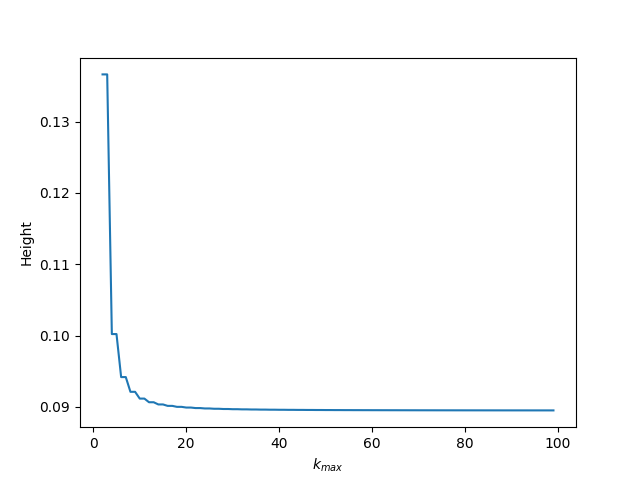
\includegraphics[width=8cm]{img/ex_6_a.png}
	\centering
\end{figure}

\lstinputlisting[language=Python, firstline=30]{code/ex_6.py}

\begin{figure}[H]
	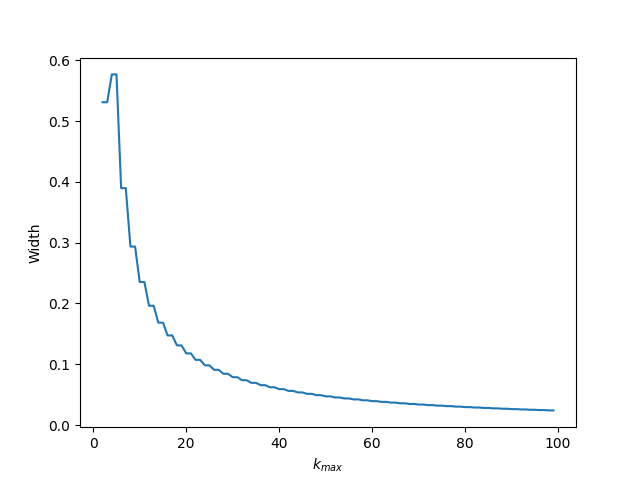
\includegraphics[width=8cm]{img/ex_6_b.png}
	\centering
\end{figure}






\newpage

\textbf{\large 7. Proof the modulation theorem}
\\

Given That:

\begin{align}
	F(x(t)) &= \int_{-\infty}^\infty x(t) e^{-i \omega t} dt \\
	\cos(\omega_0 t) &= \frac{e^{i \omega_0 t} + e^{-i \omega_0 t}}{2}
\end{align}

Follows:

\begin{align*}
	F(x(t) \cos(\omega_0 t)) &= \int_{-\infty}^\infty x(t) \cos(\omega_0 t) e^{-i \omega t} dt \\
	&= \int_{-\infty}^\infty x(t) \frac{e^{i \omega_0 t} + e^{-i \omega_0 t}}{2} e^{-i \omega t} dt \\
	&= \frac{1}{2} \left[ \int_{-\infty}^\infty x(t) e^{i \omega_0 t} e^{-i \omega t} dt + \int_{-\infty}^\infty x(t) e^{-i \omega_0 t} e^{-i \omega t} dt \right] \\
	&= \frac{1}{2} \left[ F\left[x(t) e^{i \omega_0 t} \right] + F\left[x(t) e^{-i \omega_0 t} \right] \right] \\
	&= \frac{1}{2} \left[ X(\omega - \omega_0) + X(\omega + \omega_0) \right]
\end{align*}



\textbf{\large 8. sinc-function}
\\

\textbf{
	a) Show that the spectral density of the sinc-function is a boxcar. 
} 
\\

Given that:

\begin{align}
	\sin(x) &= \frac{1}{2i} \left( e^x - e^{-x} \right) \\
	\text{sinc}(x) &= \frac{\sin(x)}{x}
\end{align}

Follows:

\begin{align*}
	x(t) &= \frac{1}{2 \pi} \int_{-\infty}^{\infty} e^{i \omega t} d \omega 
	= \frac{1}{2 \pi} \int_{-W}^{W} e^{i \omega t} d \omega 
	= \frac{1}{2 \pi i t} \left( e^{i W t} - e^{-i W t} \right) \\
	&= \frac{W}{\pi W t} \sin(W t) 
	= \frac{W}{\pi} \text{sinc}(W t) \\ 
\end{align*}

\textbf{
	b) What is the relation of the distance between the zero crossings of the sinc to the width of the boxcar? 
	Specifically, what happens for very dense/very sparse zero crossings?
}
\\

Given that $2W$ represents the width of the boxcar function follows:

\begin{align*}
	x(t) &= \frac{W}{\pi} \text{sinc}(W t) = \frac{\sin(W t)}{\pi t}\\ 
	&\Rightarrow x(t) = 0\ \forall\ t \in \left\{n \frac{\pi}{W}\ |\ n \in \mathbb{Z} \setminus \{0\} \right\} \\
	&\implies l_0 = \frac{\pi}{W}
\end{align*}

The distance between zero crossings $l_0$ is inverse proporitional to the width of the boxcar $2W$.


\newpage
\textbf{\large 9. Signal Digitization}
\\

\lstinputlisting[language=Python, firstline=0,
	caption=Python code for exercise 9
]{code/ex_9.py}

\begin{figure}[H]
	\centering
	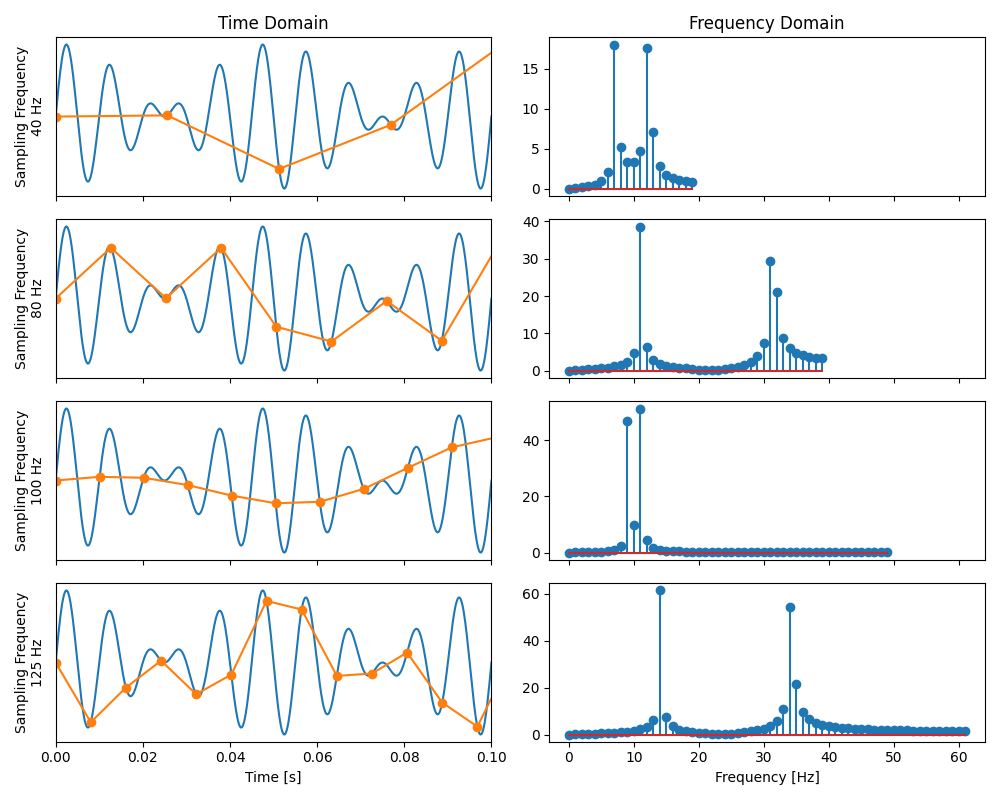
\includegraphics[width=16cm]{img/ex_9.png}
	\captionsetup{width=14cm}
	\caption{Plot for exercise 9. The given signal sampled at different rates, visualized in the time and frequency domain.}
\end{figure}


%\textbf{\large 11. FIR filters}
%\\
%
%\begin{align}
%	H(\omega) &= \sum_{n=-\infty}^\infty h_n e^{-i \omega n} \\
%	&= h_{-1} e^{i \omega} + h_0 e^{0} + h_1 e^{-i \omega} \\
%	&= h_0 + h_1 \left( e^{i \omega} + e^{-i \omega} \right) & & \text{with}\ h_{-1} = h_1 \\
%	&= h_0 + 2 h_1 \cos(\omega) \\
%\end{align}
%
%
%\textbf{a)} $\{h_{-1}, h_0, h_1\} = \left\{\frac{1}{3}, \frac{1}{3}, \frac{1}{3}\right\}$
%
%\begin{equation*}
%	H(\omega) = \frac{1}{3} + \frac{2}{3} \cos(\omega)
%\end{equation*}
%
%\textbf{b)} $\{h_{-1}, h_0, h_1\} = \left\{\frac{1}{4}, \frac{1}{2}, \frac{1}{4}\right\}$
%
%\begin{equation*}
%	H(\omega) = \frac{1}{2} + \frac{1}{2} \cos(\omega)
%\end{equation*}
%
%\textbf{c)} $\{h_{-1}, h_0, h_1\} = \left\{-\frac{1}{4}, \frac{1}{2}, -\frac{1}{4}\right\}$
%
%\begin{equation*}
%	H(\omega) = \frac{1}{2} - \frac{1}{2} \cos(\omega)
%\end{equation*}
%
%\vspace{1cm}
%Since all filters are symmetric around the orgin, the phase is zero.
%
%\begin{figure}[h]
%	\centering
%	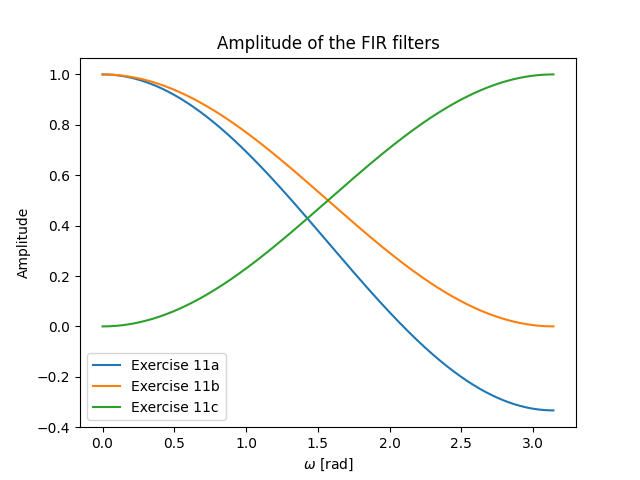
\includegraphics[width=12cm]{img/ex_11.png}
%	\captionsetup{width=10cm}
%	\caption{Amplitudes for the given FIR filters.}
%\end{figure}


\textbf{\large 12. Multipying frequency responses}
\\

\textbf{a) Amplitude Plot}\\

Given that:

\begin{align}
	H_b(\omega) &= \frac{1}{4} + \frac{1}{2} \cos(\omega) \\
	H_c(\omega) &= \frac{1}{4} - \frac{1}{2} \cos(\omega) \\
	\cos^2(x) &= \frac{1+\cos(x)}{2}
\end{align}

Follows:

\begin{align*}
	H_{bc}(\omega) &= H_b(\omega) H_c(\omega) \\
	&= \frac{1}{4} + \frac{1}{2} \cos(\omega) - \frac{1}{2} \cos(\omega) - \frac{1}{4} \cos^2(\omega)\\
	&= \frac{1}{4} - \frac{1}{4} \cos^2(\omega) \\
	&= \frac{1}{4} - \frac{1}{4} \frac{1+\cos(2\omega)}{2} \\
	&= \frac{1}{4} - \frac{1}{8} - \frac{1}{8}\cos(2\omega) \\
	&= \frac{1}{8} - \frac{1}{8} \cos(2\omega) \\
	&= \frac{1}{8} \left(1 - \cos(2\omega)\right)
\end{align*}

\begin{figure}[h]
	\centering
	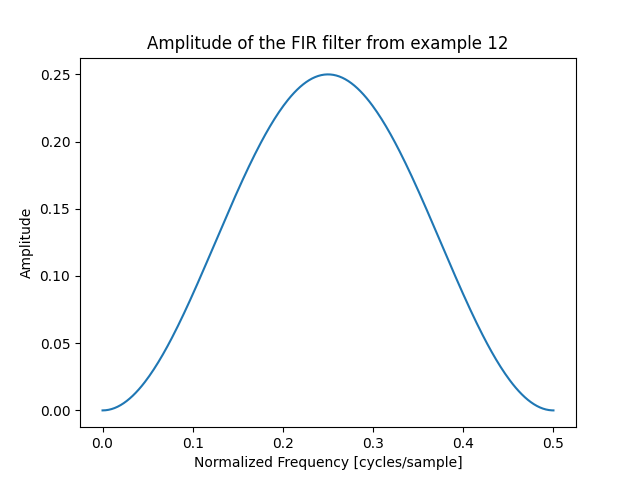
\includegraphics[width=7cm]{img/ex_12.png}
	\captionsetup{width=5cm}
	\caption{Amplitude for the given FIR filters.}
\end{figure}

\newpage

\textbf{b) Time Domain Coefficiants} \\

Given that:

\begin{align}
	H_{bc}(\omega) &= \frac{1}{8} - \frac{1}{8} \cos(2\omega) \\
	\cos(x) &= \frac{e^x + e^{-x}}{2}
\end{align}

Follows:

\begin{align*}
	\frac{1}{8} - \frac{1}{8} \cos(2\omega) &= \frac{1}{8} - \frac{1}{8} \frac{e^{2i\omega} + e^{-2i\omega}}{2} \\ 
	&= -\frac{1}{16} e^{2i\omega} + \frac{1}{8} e^{0i\omega} - \frac{1}{16} e^{-2i\omega} \\
	&\Rightarrow \left\{ -\frac{1}{16},\ 0,\ \frac{1}{8},\ 0,\ -\frac{1}{16} \right\}
\end{align*}

\textbf{\large 13. IRR filter}
\\

Given that:

\begin{align}
	\{a_{-1},\ a_0,\ a_1\} &= \left\{-\frac{1}{2},\ 1,\ 0\right\} \\
	\{b_{-1},\ b_0,\ b_1\} &= \left\{\frac{1}{8},\ \frac{1}{4},\ \frac{1}{8}\right\}
\end{align}
Follows:

\begin{align*}
	H(\omega) &= \frac{Y(\omega)}{X(\omega)}\\
	&= \frac{\frac{1}{8} e^{i\omega} + \frac{1}{4} + \frac{1}{8} e^{-i\omega}}{-\frac{1}{2} e^{i\omega} + 1}\\
	&= \frac{\frac{1}{4} (1 + cos(\omega))}{1 - \frac{1}{2} e^{i\omega}}
	&= \frac{1 + cos(\omega)}{4 - 2 e^{i\omega}}
\end{align*}

\begin{figure}[h]
	\centering
	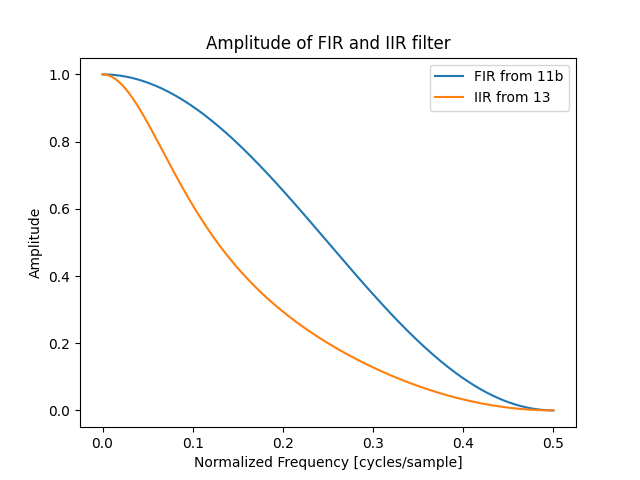
\includegraphics[width=8cm]{img/ex_13.png}
	\captionsetup{width=6cm}
	\caption{Amplitude comparison for the filters from example 11a and 13.}
\end{figure}


\newpage
\textbf{\large 15. Frequency Response of Laplace domain signals}
\\

\lstinputlisting[language=Python, firstline=0,
	caption=Python code for exercise 15
]{code/ex_15.py}

\begin{figure}[H]
	\centering
	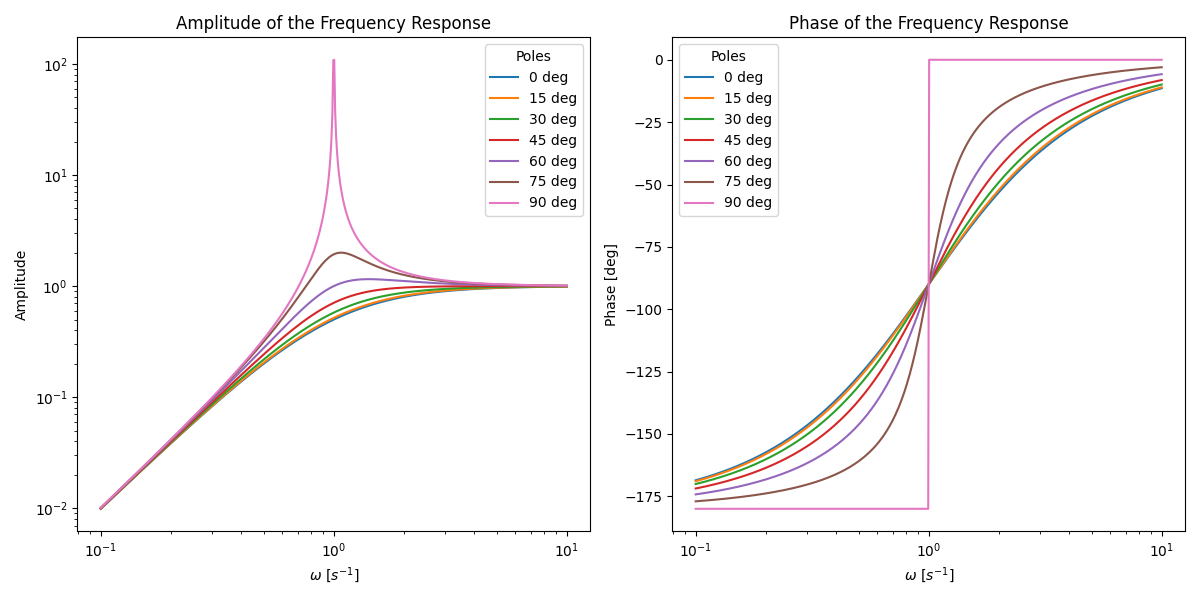
\includegraphics[width=16cm]{img/ex_15.png}
	\captionsetup{width=14cm}
	\caption{Plot for exercise 15. The amplitude and phase of the frequency response of signals with different pole angles.}
\end{figure}


\end{document}
